\documentclass[10pt]{article}
\usepackage{float}
\usepackage{listings}
\usepackage[french]{babel}
\usepackage[utf8x]{inputenc}
\usepackage{subcaption}
\usepackage{listings}
\usepackage{color}
\usepackage{amsmath}
\usepackage{amsfonts}
\usepackage{mathtools}
\usepackage{graphicx}
\usepackage{caption}
\definecolor{dkgreen}{rgb}{0,0.6,0}
\definecolor{gray}{rgb}{0.5,0.5,0.5}
\definecolor{mauve}{rgb}{0.58,0,0.82}
%opening

\lstset
{frame=tb,
	language=R,
	aboveskip=3mm,
	belowskip=3mm,
	showstringspaces=false,
	framexleftmargin=5mm,
	columns= fixed,
	numbers = left,
	basicstyle={\small\ttfamily},	
	numberstyle=\tiny\color{gray},
	keywordstyle=\color{blue},
	commentstyle=\color{dkgreen},
	stringstyle=\color{mauve},
	breaklines=true,
	breakatwhitespace=true,
	tabsize=3
}


\title{
	\normalfont \normalsize 
	\textsc{Université de Technologie de Compiègne\\ 
		SY09:Analyse des données et Data-Mining , P17} \\
	[10pt] 
	\rule{\linewidth}{0.5pt} \\[6pt] 
	\huge Premier Rendu \\
	\rule{\linewidth}{2pt}  \\[10pt]
}
\author{Oumaima Talouka, Zineb Slam}
\date{\normalsize \today}

\begin{document}
	
{\let\newpage\relax\maketitle}

Dans ce rapport du TP1 de l'UV SY09 nous allons expliquer notre démarches dans l'analyse des données en expliquant les résultats obtenus. Ce TP est compose de 2 parties. La première partie a pour objectif de se familiariser avec les méthodes de traitement et de visualisation de données sur R. La deuxième partie traite de l'Analyse en composantes principales (ACP). Nous allons travailler avec 3 dataset notes de SY02, Crabs et Pima qu'on va d'abord analyser et décrire avant d'y réaliser l'ACP en seconde partie. Pour les graphes obtenus nous avons utilises la librairie ggplot2 qui offre un grand nombre de fonctionnalité Le code R sera fourni en annexe.



\tableofcontents


\section{ Statistique descriptive}

\subsection{Notes SY02}
Le dataset \textit{"sy02-p2016"} représente les notes des étudiants de l'UTC en méthodes statistiques durant le printemps 2016. Nos données comptent \textit{N= 296} individus (étudiants) er \textit{p= 11} variables. Nous avons omis  les etudiants qui n'avaient pas de résultats (\textit{NA}) ou qui ont '\textit{ABS}' en résultat de l'UV parce que ce qu'on a pense que ce sont des etudiants qui s'étaient de-inscris ou n'ont pas suivi l'UV et donc ne constituent pas d'information pour notre dataset. Nous gardons néanmoins les etudiants qui ont NA en médian ou en final mais qui ont obtenu un résultat final. 

\begin{lstlisting}
dataset = dataset[!is.na(dataset$resultat), ]
dataset = dataset[dataset$resultat!='ABS', ]
\end{lstlisting}
>>>>>>> origin/master

\section{Notes SY02}
Le dataset \textit{"sy02-p2016"} représente les notes des étudiants de l'UTC en SY02 ( statistiques) durant le printemps 2016. Nos données comptent \textit{N= 296} individus (étudiants) er \textit{p= 11} variables.  \textbf{Enlever les etudiants desinscrits}

 \subsection{Description des variables}

\begin{center}
	\begin{tabular}{c c }
		\textbf{Variables Quantitatives} & note.median, note.final, note.totale \\ 
		 \textbf{Variables Qualitatives Nominales} & nom, specialite, status, dernier.diplome.obtenu, correcteur.median, correcteur.final\\
		  \textbf{Variables Qualitatives Ordinales}  & niveau, et rltat  \\
	\end{tabular}
	\captionof{table}{Categorie de Variables}
\end{center} 

 Nous allons a présent définir  chaque variable en précisant son intervalle ou les valeurs qu'elle peut prendre.

\begin{itemize}
	\item \textbf{Nom:} chaine de caractère identifiant chaque étudiant.
	\item \textbf{Spécialité:} la branche de l'étudiant: \textit{GB}, \textit{GM}, \textit{GSM}, \textit{GP} et \textit{GI}.
	\item \textbf{Niveau}: Semestre d'étude de chaque étudiant de 1 a 6.
	\item \textbf{Statut}: Soit l'étudiant est de l'\textit{UTC} ou en s\textit{emestre d'échange}
	\item \textbf{dernier.diplome.obtenu:}
	\textit{BAC, DUT, CPGE, ETRANGER SUPERIEUR, LICENCE, OTHER, NA}
	\item \textbf{Note Médian:} note de l'examen Médian, ensemble de réel de 0 a 20.
	\item \textbf{Correcteur Médian:} ID du correcteur du médian \{Corr1, Corr2, Corr4., Corr5,..,Corr8\}
	\item \textbf{Note.final:} Note de l'examen final, ensemble de réel de 0 a 20.
	\item \textbf{Note.totale:} Note totale obtenue a partir de la note du médian et la note du final
	\item \textbf{Correcteur.final}: identifiant  du correcteur du final. \{Corr1..Corr3, Corr4., Corr5,..,Corr8\}
	\item \textbf{Résultat}: Résultat obtenu en SY02 : \textit{A, B, C, D, E et FX et FX. ABS}. ABS est pour indiquer que l'étudiant était absent pour l'examen en question.
\end{itemize}

Pour les notes de médian et de final il y'a des notes non mentionnées (NA) par contre tous les etudiants ont un résultat final c'est pour cela on n'a pas enlevé les etudiants avec NA en médian ou/et en final.\\
Les variables importantes dans ce dataset sont les résultats des etudiants et comment ceux ci sont influences par d'autre variable, par exemple le niveau et la spécialité\\
Il est évident qu'il existe une relation linéaire entre ces 3 variables: note.median, note.final et note.totale vu que la note totale est exprimée par une relation linéaire entre la note.median et la note.final (par exemple $note.totale = 40\% * note.median + 40\% * note.final + cste$). La variable note.totale et la variable resultat sont des variables fortement corrélés En effet le résultat est une "traduction"  de la note totale. On pourrait éventuellement se demander sur la relation entre les notes et le niveau, la spécialité, le diplôme ainsi que le correcteur. C'est ce qu'on va essayer d'analyser dans ce qui suit. 


\subsubsection{Liens entre les variables}
Après avoir représenté la matrice de graphes pour chaque variable nous avons pu observe que les variables : note.median, note.final, et note.totale sont linéaire ce qui confirme note hypothèse précédente Le graphe matriciel ci-dessous présente aussi les coefficients de corrélation entre chacune de ces variables.
>>>>>>> origin/master

\subsubsection{Lien entre les variables}
	\begin{center}
	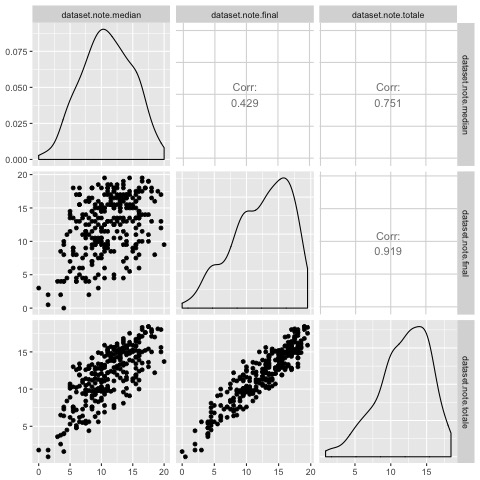
\includegraphics[width=50mm]{Figures/Notes/corr_notes.jpg}
	\captionof{figure}{Plot general}
	\label{fig:multiplot_notes}
\end{center}


\subsubsection{Homogénéité et Distribution des notes}
La figure ci-dessous représente trois diagrammes a boites des notes de médian, final et le résultat de l'UV SY02. 

\begin{minipage}{.4\textwidth}	
	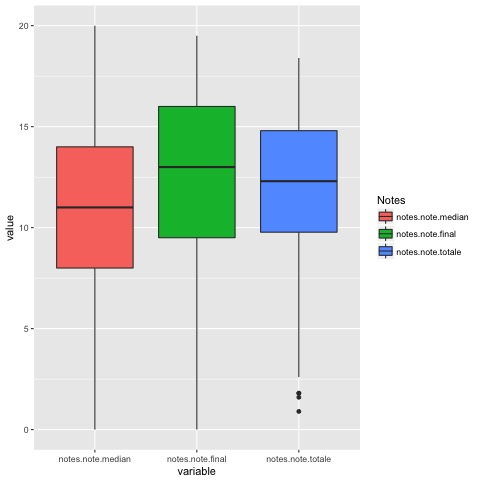
\includegraphics[width=55mm]{Figures/Notes/boxplot_exam.jpg}
	\captionof{figure}{Boxplot des Notes }
	\label{fig:Boxplot_notes}
\end{minipage}%
\hspace{0.03\linewidth}
\begin{minipage}{.6\textwidth}
	\begin{tabular}{ c c c c }
		\textbf{}       & \textbf{Médian} & \textbf{Final}   & \textbf{Total} \\
		\textbf{1er Quartl}    & 8.0 			       & 9.50		      & 9.77    \\
		\textbf{Médiane  }   &11.0		             & 13.0	            & 12.3    \\
		\textbf{Moyenne}     & 10.92                &  12.38          & 11.84\\
		\textbf{3em Quartl}  & 14.0  				& 16.0 		       & 14.8\\
	\end{tabular}
\end{minipage}
>>>>>>> origin/master

Il est tout a fait logique que le digramme de résultats se situe entre les 2 puisque que c'est la moyenne \textbf{pondérée??} des 2deux notes du médian etfinal.                              en entre la réussite, la formation, la branche et le niveau

On remarque les boites sont petites ce qui laisse penser que la variance des résultats est relativement petite et donc aussi que le niveau des etudiants en statistiques l'est aussi.  En comparant les diagrammes du final et du médian on remarque que les notes ont augmente.  Enfin si on analyse le dernier diagramme on voit que les deux boites du part et d'autre de la médiane ont la même taille, on peut donc mettre l'hypothèse que les résultats sont normalement distribués. 

Il est tout a fait logique que le digramme de boites des notes finales se situe entre les 2 puisque que la note finale est une moyenne des deux notes du médian et du final.
 
	
\subsubsection{Lien entre la réussite, la formation, la branche et le niveau}
Comme les etudiants de chaque branche n'ont pas les \textit{même effectifs} on a choisi de représenter les données sous forme de diagrammes de moustache pour mieux pouvoir les comparer.\\


	\begin{minipage}{.5\textwidth}
		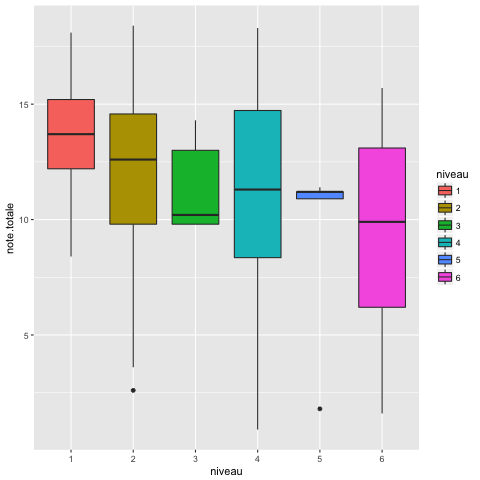
\includegraphics[width=50mm]{Figures/Notes/niveau_resultat.png}
		\captionof{figure}{Diagramme en boite de lien entre le niveau et le resultat}
		\label{fig:niveau_resultat}
	\end{minipage}%
	\hspace{0.08\linewidth}
	\begin{minipage}{.5\textwidth}
		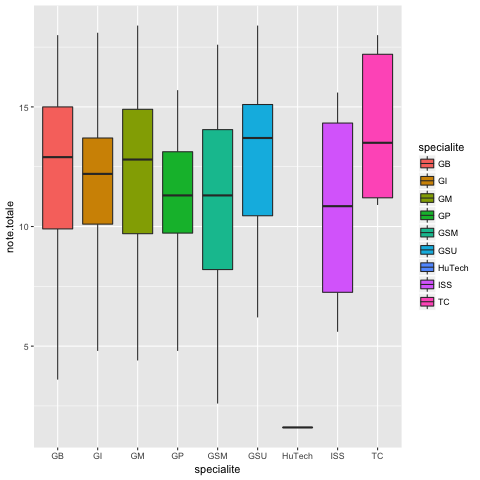
\includegraphics[width=50mm]{Figures/Notes/specialite_resultat.png}
		\captionof{figure}{Diagramme en boite de lien entre la branche et le resultat}
		\label{fig:specialite_resultat}
	\end{minipage}
D'après la figure \ref{fig:niveau_resultat} on remarque que les etudiants venant durant les premiers semestres sont ceux qui réussissent le mieux leur examens de SY02 , suivi par ceux en GX02. On remarque que les notes des etudiants en GX04 et GX05 ont une grande variance. Les étudiants en GX04 et en GX05 ont . Il faut aussi remarquer que les étudiants en 4em et 5 em sont peu comme c'est des semestres de départ en stage. \\
En ce qui concerne l'influence de la spécialité sur les notes on remarque qu'il y'a une grande variance dans les  notes chez les etudiants en  TC et ISS et GSM, contrairement au GI et GP qui ont plutôt un niveau homogène et qui semble bien réussir l'UV. De plus les TC sont aussi ceux qui réussissent le mieux l'UV.
\begin{center}
	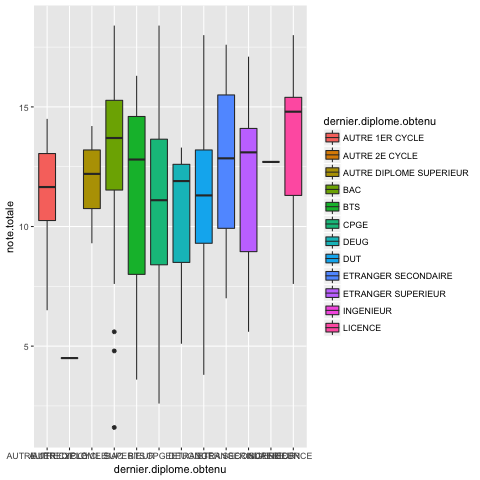
\includegraphics[width=50mm]{Figures/Notes/diplome_resultat.png}
	\captionof{figure}{Diagramme de moustache de lien entre la formation et le resultat}
	\label{fig:formation_resultat}	
	\end{center}

		On remarque qu'il y'a une grande variance chez  presque tous les diplômes obtenus. Les élèves qui réussissent le mieux et le plus sont ceux provenant de la Licence.  Plus de 75\%  (\textbf{Check}) des etudiants de autre premier  cycle et autres diplômes et  du BAC réussissent l'UV SY02. En ce qui concerne les résultats des etudiants pour le reste des diplômes ils ont une grande variance et ne sont pas normalement distribues. En particulier les etudiants du BTS, CPGGE et du DEUG sont ceux qui ont la plus grande variance et le plus grand échec.


\subsubsection{Influence du correcteur sur la note}

\begin{minipage}{\linewidth}
	Les deux diagrammes ci-dessous montrent la dispersion des notes de final et de médian pour chaque correcteur.\\
	\begin{minipage}{0.50\linewidth}
	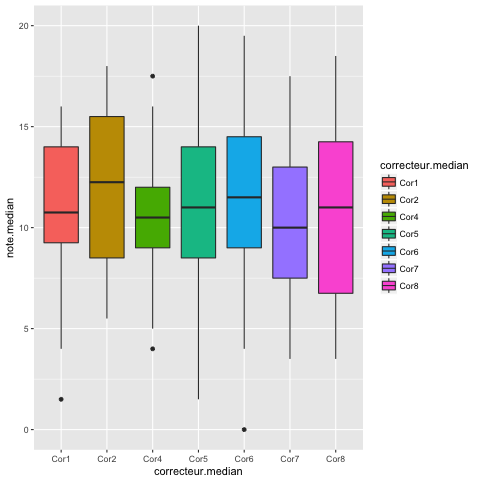
\includegraphics[width=50mm]{Figures/Notes/correcteur_median.png}
	\captionof{figure}{Diagramme de moustache des notes de median en fonction des correcteurs}
	\label{fig:scatter_correcteur_median}
	\end{minipage}
	\hspace{0.01\linewidth}
	\begin{minipage}{0.50\linewidth}	
		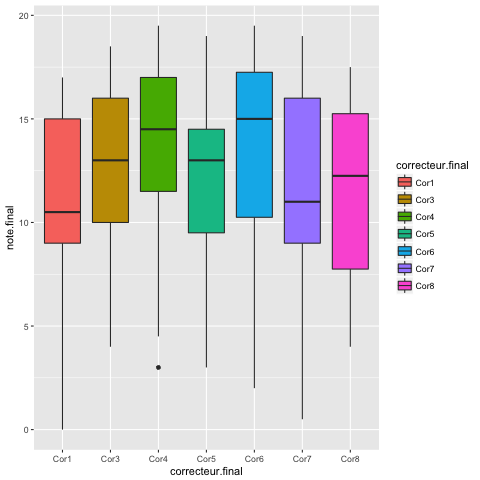
\includegraphics[width=50mm]{Figures/Notes/correcteur_final.png}
		\captionof{figure}{Diagramme de moustache des notes du final en fonction des correcteurs}
		\label{fig:scatter_correcteur_median}
	\end{minipage}
\end{minipage}
on considère que les copies sont aléatoirement distribues pour chaque correcteur et donc il n' y'a pas de correcteur qui a que les 'bons' ou les 'mauvais' étudiants A première vue on remarque qu'en général les notes sont dispersées pour chaque correcteur et donc il n y'a pas vraiment de correcteur en particulier qui semble être plus 'sévère' que les autres. On peut emmètre l'hypothèse  que le \textit{Corr4} a été plus stricte dans ses corrections de médians, néanmoins son diagramme de notes de final prouve le contraire. Il se peut donc que le correcteur avait les copies des 'mauvais' etudiants par fruit de hasard. Finalement, comme il a été cite précédemment les notes ont augmente au final par rapport au médian, on observe donc bien que ceci est le cas pour tous les correcteurs.

\subsubsection{Conclusion}
Cette première analyse data nous a permis d'étudier  quels sont les facteurs qui influent sur la réussite d'un étudiant dans l'UV SY02 comme le dernier diplôme obtenu ou le niveau et ceux qui n' influence pas comme le correcteur. Néanmoins ces conclusions sont \underline{propre a la population du P16} et donc  \underline{biaisées}; pour pouvoir généraliser il faut analyser les notes de SY02 sur plusieurs semestres avec des populations différentes.
>>>>>>> origin/master

\section{Crabs}
Le dataset \textit{"Crabs"} représente un jeu de données de 200 crabes décrits par huit variables, trois sont qualitatives et cinq sont quantitatives.

\subsection{Description des variables}


\begin{itemize}
	\item \textbf{Variables Qualitatives Nominales :}  crabs.sp, crabs. sex, crabs.inde
	\item \textbf{Variables Quantitatives : } crabs.FL, crabs.RW, crabs.CL, crabs.CW, crabs.BD
\end{itemize}

Nous pouvons représenter les données des variables quantitatives a l'aide un boxplot.
\begin{center}
	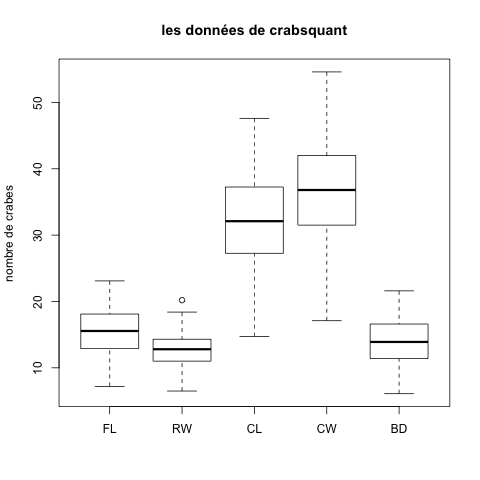
\includegraphics[width=50mm]{Figures/Crabs/bxp_crabsquant.png}
	\captionof{figure}{Boxplot des données quantitaves}
	\label{fig:boxplot_crabs_quantitatives}
\end{center}

Nous remarquons d'ores et deja que deux categories de variables se distinguent, d'un cote FL, RW et BD et d'un autre, CL et CW.

Avant de continuer l'analyse de ces donnees, nous pouvons preciser la signification de chacune de ces variables comme suit:
\begin{itemize}
	\item \textbf{sp:} \textit{(species)}, espece, "B" pour Bleu et "O" pour Orange
	\item \textbf{sex:} sexe, "F" pour Feminin et "M" pour masculin
	\item \textbf{index:} index de 1 a 50 pour chacune des 4 categories suivantes : \{"B,M","O,M","B,F","O,F"\}
	\item \textbf{FL:} Frontal Lobe size en mm
	\item \textbf{RW:} Rear Width en mm
	\item \textbf{CL:} Carapace Length en mm
	\item \textbf{CW:} Carapace Width en mm 
	\item \textbf{BD:} Body Depth en mm
\end{itemize}

\subsection{Analyse descriptive des données}

\subsubsection{Représentation de chaque caractéristique en fonction de l'espèce}

Afin de voir s'il y a une différence de caractéristiques morphologiques en fonction de l'espèce d'abord, nous représentons les boites a moustache de chaque variable morphologique en fonction de la variable sp comme suit:

\begin{center}
	\begin{minipage}[t]{0.3\textwidth}
		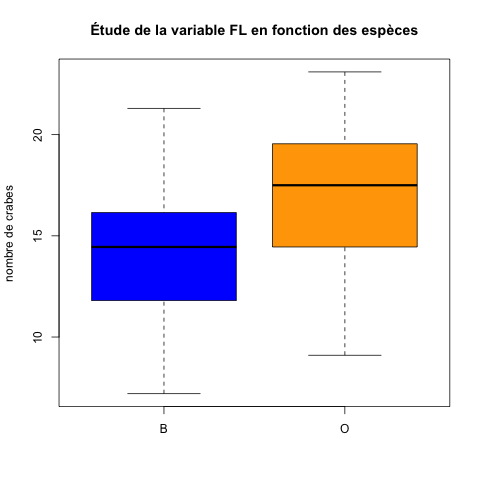
\includegraphics[width=35mm]{Figures/Crabs/bxp_sp_fl.png}
	\end{minipage}
	\begin{minipage}[t]{0.3\textwidth}
		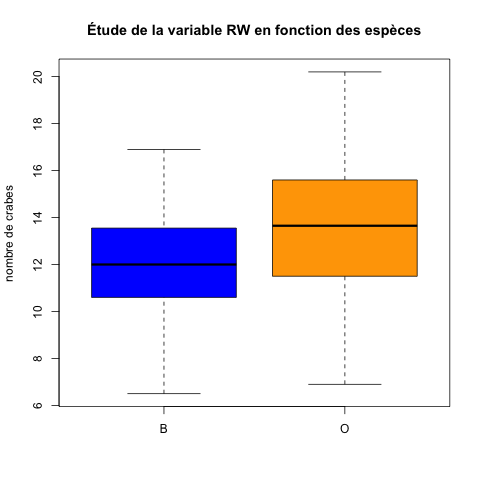
\includegraphics[width=35mm]{Figures/Crabs/bxp_sp_rw.png}	
	\end{minipage}
	\begin{minipage}[t]{0.3\textwidth}
		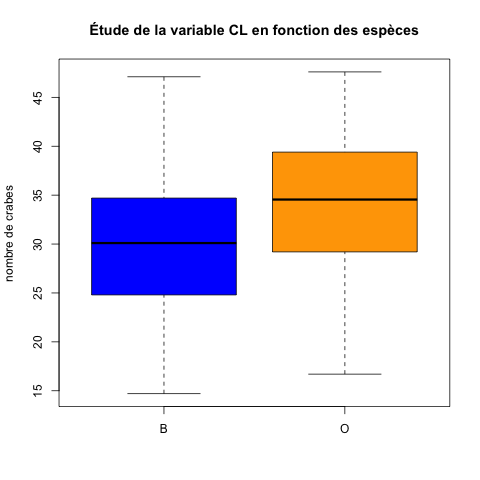
\includegraphics[width=35mm]{Figures/Crabs/bxp_sp_cl.png}
	\end{minipage}
	\newline
	\begin{minipage}[t]{0.3\textwidth}
		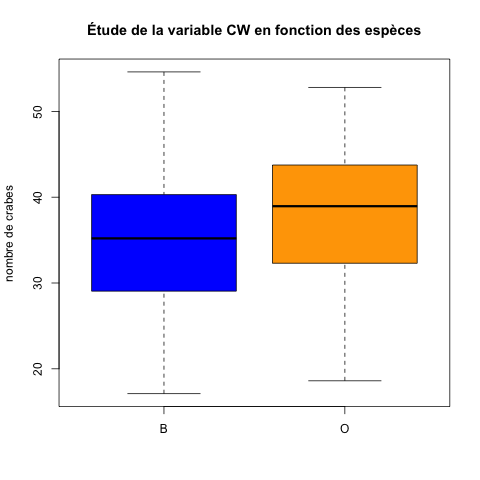
\includegraphics[width=35mm]{Figures/Crabs/bxp_sp_cw.png}	
	\end{minipage}
	\begin{minipage}[t]{0.3\textwidth}
		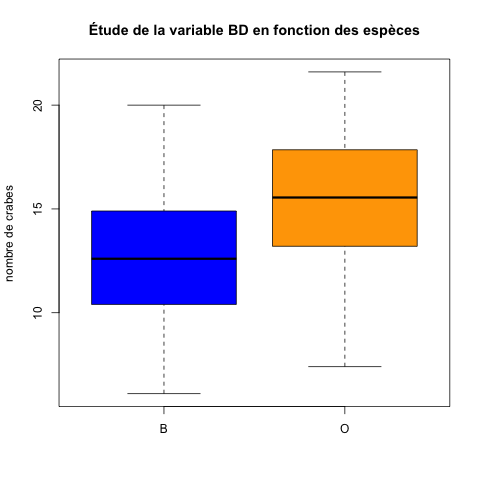
\includegraphics[width=35mm]{Figures/Crabs/bxp_sp_bd.png}
	\end{minipage}
\end{center}

Il y a des distributions assez differentes en fonction de l'espece. Les intervalles de confiances ne se chevauchent pas . Cependant, la dispersion des donnees reste assez homogene au vue des boxplots.
\subsubsection{Representation de chaque caracteristique en fonction du sexe}

Afin de voir s'il y a une difference de caracteristiques morphologiques en fonction du sexe, nous representons les boites a moustache de chaque variable morphologique en fonction de la variable sex comme suit:

\begin{center}
	\begin{minipage}[t]{0.3\textwidth}
		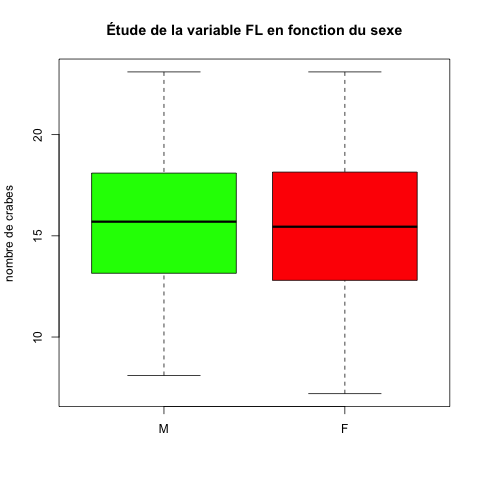
\includegraphics[width=35mm]{Figures/Crabs/bxp_sex_fl.png}
	\end{minipage}
	\begin{minipage}[t]{0.3\textwidth}
		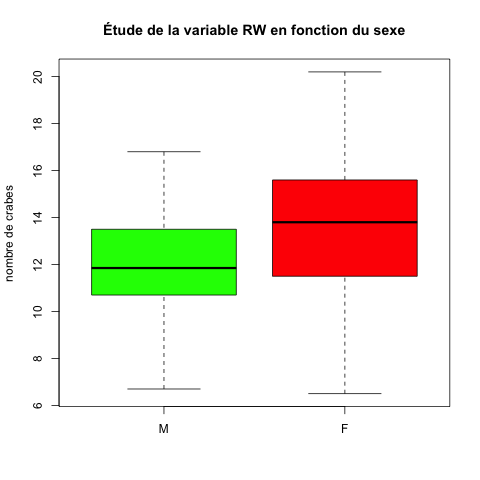
\includegraphics[width=35mm]{Figures/Crabs/bxp_sex_rw.png}	
	\end{minipage}
	\begin{minipage}[t]{0.3\textwidth}
		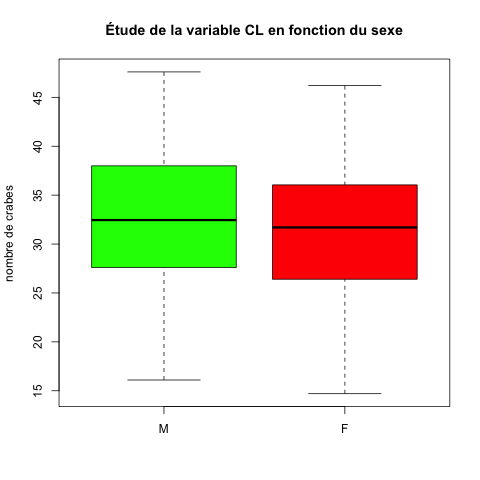
\includegraphics[width=35mm]{Figures/Crabs/bxp_sex_cl.png}
	\end{minipage}
	\newline
	\begin{minipage}[t]{0.4\textwidth}
		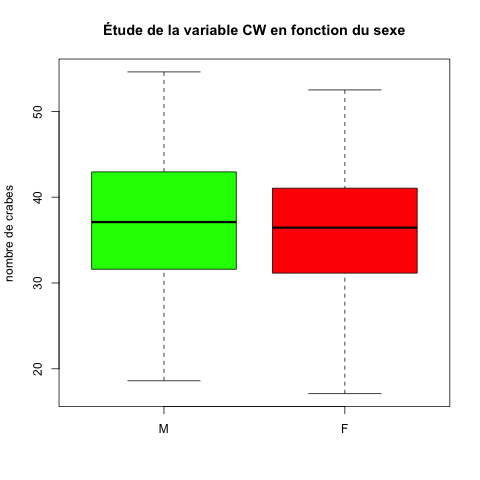
\includegraphics[width=35mm]{Figures/Crabs/bxp_sex_cw.png}	
	\end{minipage}
	\begin{minipage}[t]{0.4\textwidth}
		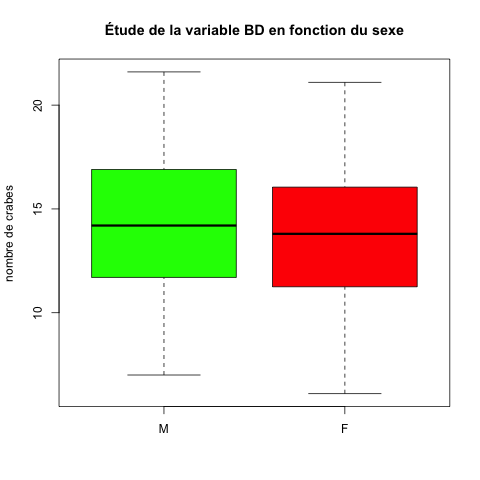
\includegraphics[width=35mm]{Figures/Crabs/bxp_sex_bd.png}
	\end{minipage}
\end{center}

A l'oppose des boxplot en fonction de l'espèce, ceux en fonction du sexe relèvent une similitude de la distribution des différentes caractéristiques pour la plupart, ainsi que la dispersion des données Nos observons que la variable RW se distingue des autres avec un largeur de l'arrière importante chez les femmes que chez les hommes.

Enfin, la nature de l'espèce impacte les caractéristiques morphologiques, a la différence du sexe, qui lui n'influe que peu ces caractéristiques
\subsubsection{Lien entre les variables}
%\begin{center}
%	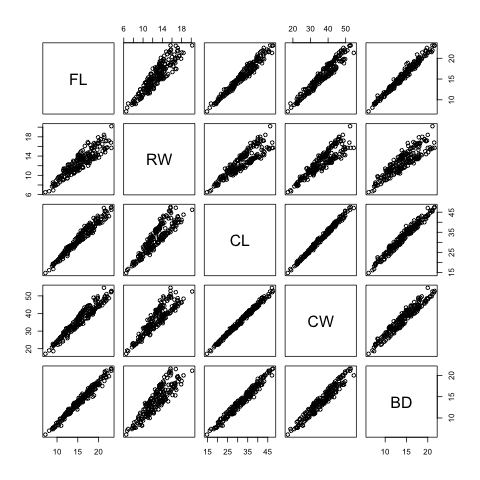
\includegraphics[width=50mm]{Figures/Crabs/plot_crabsquant.png}
%	\captionof{figure}{Plot general}
%	\label{fig:multiplot_crabs}
%\end{center}

Nous pouvons représenter chacune de ces variables quantitatives en fonction de l'espèce puis en fonction du sexe afin de déterminer la possibilité d'identifier l'une ou l'autre a partir des caractéristiques morphologiques. \\

\begin{minipage}[t]{0.6\textwidth}
		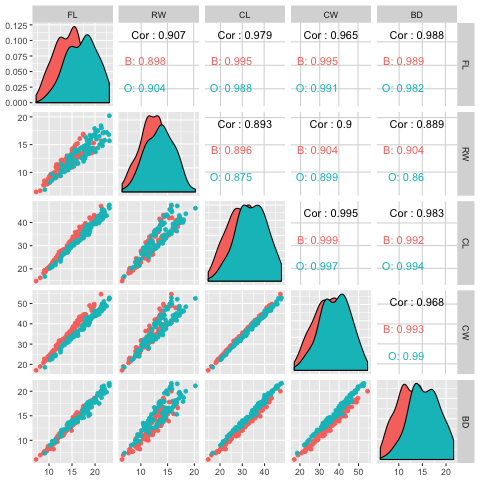
\includegraphics[width=50mm]{Figures/Crabs/matricial_plot_sp.png}
\end{minipage}
\begin{minipage}[t]{0.6\textwidth}
	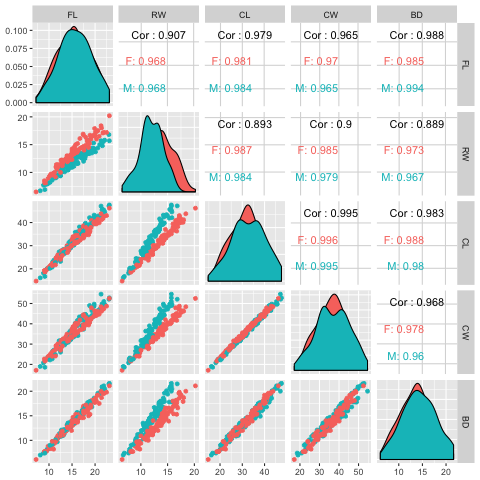
\includegraphics[width=50mm]{Figures/Crabs/matricial_plot_sex.png}
\end{minipage}
\begin{center}
	\captionof{figure}{Plot general en fonction de l'espece (gauche) et du sexe(droite)}
	\label{fig:multiplot_crabs__sp_sex}
\end{center}

Nous remarquons que ni l'espèce ni le sexe ne peuvent vraiment être identifies a partir d'une ou de plusieurs caractéristiques morphologiques.
En effet, dans les cas, l'ensemble des points est représente sur une même droite, on ne peut pas clairement distinguer l'une différence De ce fait, il est difficile de reconnaitre une espèce selon ses caractéristiques morphologiques.

\subsection{Analyse de la corrélation}

\begin{center}
	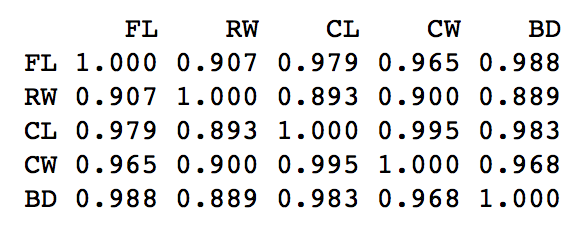
\includegraphics[width=50mm]{Figures/Crabs/cor_crabsquant.png}
	\captionof{figure}{Correlation entre les variables}
	\label{fig:cor_carbsquant}
\end{center}

Il y a une forte corrélation positive entre toutes les combinaisons de variables, telle que la valeur minimale observée est 0.889. 
Il s'agit de la taille des membres du corps d'un crabe, il semble donc logique et naturel qu'elles soient proportionnelles entre elles.
Une des façons pour s'affranchir de ce phénomène est de diviser chaque valeur par la somme totale de toutes celles de l'individu.


\section{Pima}
Le dataset \textit{"Pima"} représente un jeu de données constitue de 532 individus tous de sexe féminin décrits par huit variables dont une qualitative et sept sont quantitatives.

\subsection{Description des variables}


\begin{itemize}
	\item \textbf{Variables Qualitatives Ordinale :}  Pima.z
	\item \textbf{Variables Quantitatives : } Pima.npreg, Pima.glu, Pima.bp, Pima.skin, Pima.bmi, Pima.ped, Pima.age
\end{itemize}

Nous pouvons representer les donnees des variables quantitatives a l'aide d'un boxplot normalise de telle sorte qu'on ait toutes les variables avec une moyenne nulle et une deviation egale a 1.
\begin{center}
	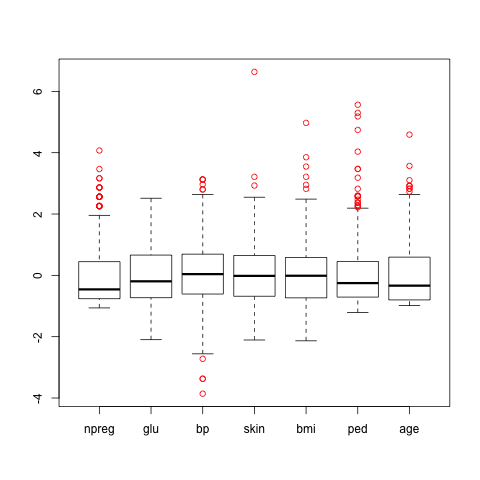
\includegraphics[width=50mm]{Figures/Pima/boxplot_norm_Pimaquant.png}
	\captionof{figure}{Boxplot normalisé des données quantitatives}
	\label{fig:boxplot_norm_pima_quantitatives}
\end{center}
D'apres les boxplots normalises, il existe plusieurs donnees aberantes. Les variables \textit{ped} et \textit{age} sont clairement pas symetriques. De plus, les distributions des differentes variables sont assez differentes du fait qu'elles ne se chevauchent pas, ainsi que l'existance de plusieurs valeurs extremes.
\begin{center}
	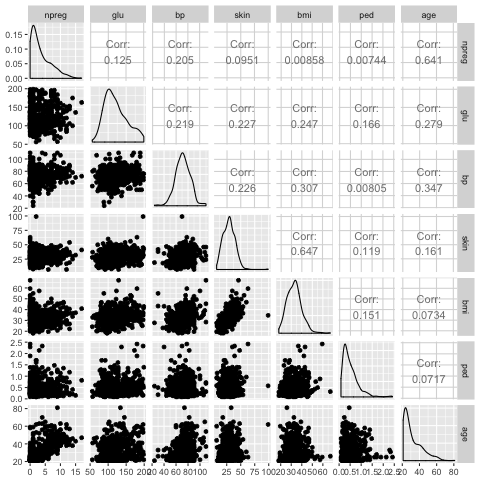
\includegraphics[width=50mm]{Figures/Pima/plot_Pimaquant.png}
	\captionof{figure}{Plot des données quantitatives}
	\label{fig:plot_pima_quantitatives}
\end{center}

Nous remarquons qu'un seul des scartterplots represente une forte association entre l'indice de masse corporelle \textit{bmi} et et l'epaisseur du pli cutane au niveau du triceps \textit{skin}.
\subsection{Analyse descriptive des données}

\subsubsection{Représentation de chaque caractéristique en fonction de z (diabétique ou pas)}

\begin{center}
	\begin{minipage}[t]{0.3\textwidth}
		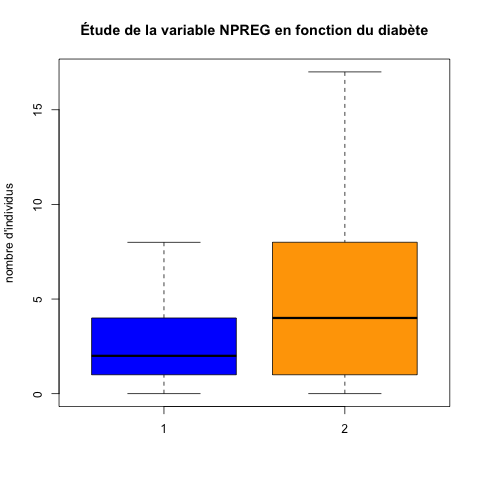
\includegraphics[width=35mm]{Figures/Pima/bxp_z_npreg.png}
	\end{minipage}
	\begin{minipage}[t]{0.3\textwidth}
		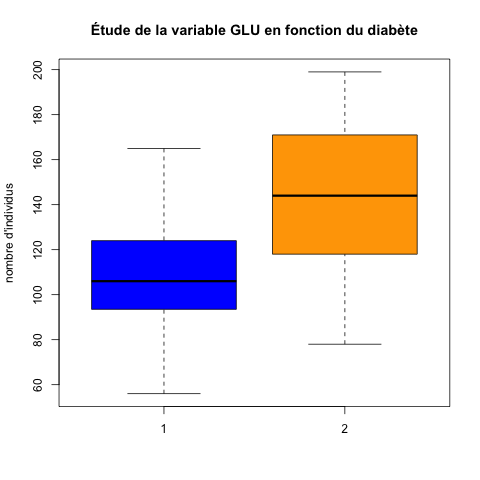
\includegraphics[width=35mm]{Figures/Pima/bxp_z_glu.png}	
	\end{minipage}
	\begin{minipage}[t]{0.3\textwidth}
		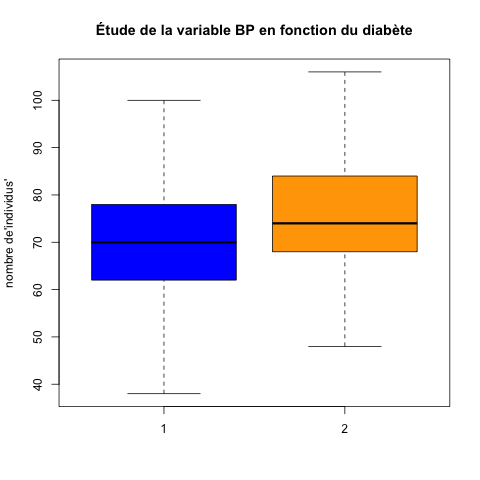
\includegraphics[width=35mm]{Figures/Pima/bxp_z_bp.png}
	\end{minipage}
	\newline
	\begin{minipage}[t]{0.3\textwidth}
		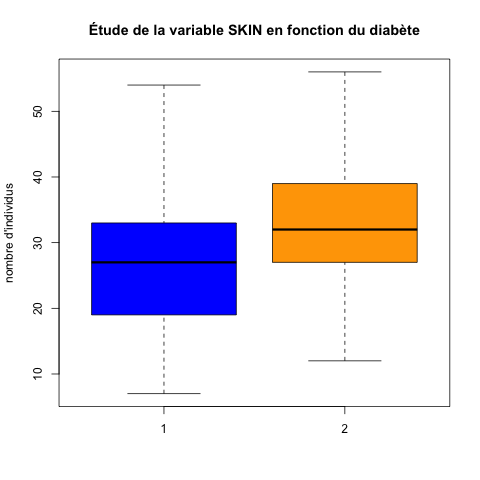
\includegraphics[width=35mm]{Figures/Pima/bxp_z_skin.png}	
	\end{minipage}
	\begin{minipage}[t]{0.3\textwidth}
		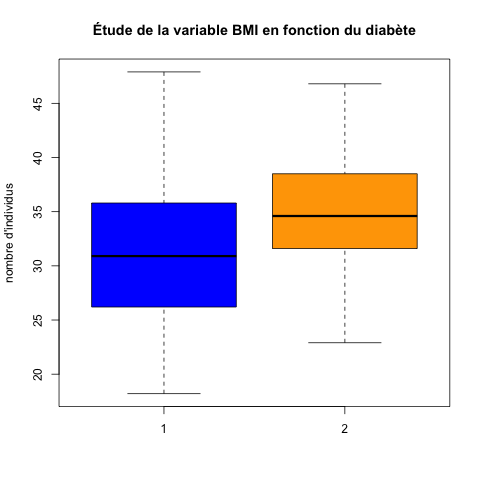
\includegraphics[width=35mm]{Figures/Pima/bxp_z_bmi.png}
	\end{minipage}
	\newline
	\begin{minipage}[t]{0.3\textwidth}
		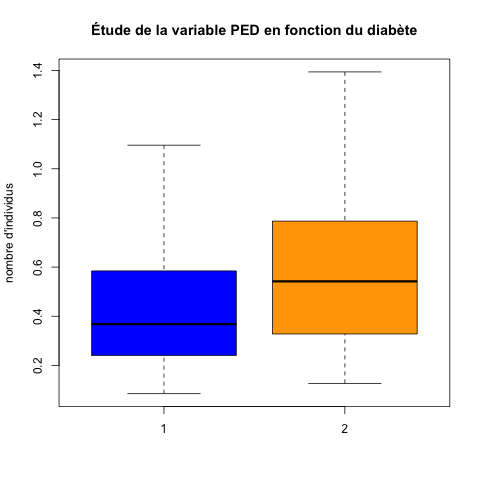
\includegraphics[width=35mm]{Figures/Pima/bxp_z_ped.png}
	\end{minipage}
	\begin{minipage}[t]{0.3\textwidth}
		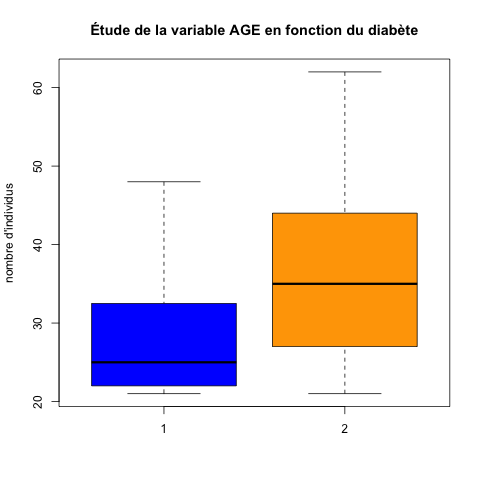
\includegraphics[width=35mm]{Figures/Pima/bxp_z_age.png}
	\end{minipage}
\end{center}

On remarque une grande difference de distributions en fonction de la categorie z. Les intervalles de confiances ne se chevauchent pas. La dispersion des donnees est aussi differentes selon chaque variable. De ce fait, le diabete (variable  qualitative) impacte considerablement chacune des variables quantitatives. 
Selon les medianes bien differentes entre les tests positifs et negatifs de diabete, nous pouvons dire que l'age par exemple, la fonction de pedegree ou encore le nombre de grossesses peut aider a estimer les resultats des tests.
Les donnees dont on dispose affirme que le diabete ne suit pas forcement la genetique, ceux dont les proches ou ancetres ont soufferts de diabete ne se sont pas forcement exposes a un risque eleve d'etre affectes eux meme. Il est important de noter que cette conclusion ne concerne que le dataset dont on dispose pour cette analyse (elle ne se reflete pas forcement sur les analyses medicale)

\subsection{Crabs}

\subsection{Pima}

\subsection{Crabs}

\subsection{Pima}
\pagebreak

\section{Analyse Composantes Principales}
Dans cette section nous allons nous concentrer sur la technique de l’Analyse en Composantes Principales qui consiste a transformer des variables corrélées en nouvelles variables non corrélées.
 \subsection{Exercice théorique}
\subsection{Utilisation des outils de R}
\subsection{Crabs}

\subsubsection{PCA}
Nous faisons appel a la fonction princomp qui calcule les composantes princpal de notre dataset. Ensuite nous utilsons le plot dans la figure \ref{fig:crabs_pca_plot} et le biplot dans la figure \ref{fig:crabs_pca_biplot}.\\
	\begin{minipage}{.5\textwidth}
		\centering
		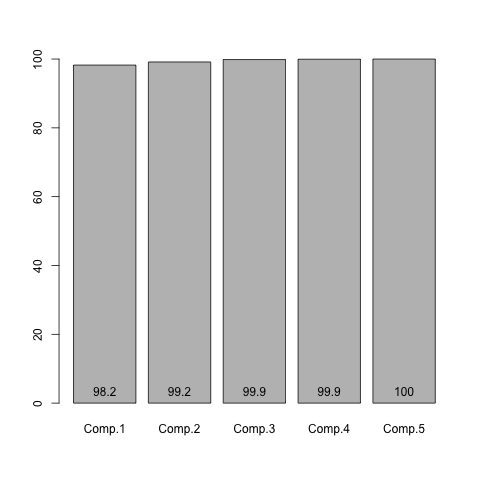
\includegraphics[width=50mm]{Figures/Crabs/pca_plot.png}
		\captionof{figure}{Variance expliquee par les composantes}
		\label{fig:crabs_pca_plot}
	\end{minipage}%
	\hspace{0.08\linewidth}
	\begin{minipage}{.5\textwidth}
		\centering
		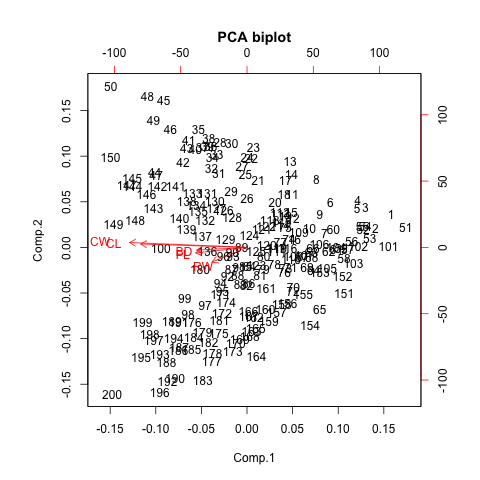
\includegraphics[width=50mm]{Figures/Crabs/pca_biplot.png}
		\captionof{figure}{Individus et Variables projetes sur le premier plan factoriel}
		\label{fig:crabs_pca_biplot}
	\end{minipage}
D'après la figure \ref{fig:crabs_pca_plot} on remarque que la première composante concentre la majorité de l'information, ceci est aussi illustrée dans la figure \ref{fig:crabs_pca_plot} puisqu'on remarque que toutes les variables ont la même direction \textbf{vers la composante 2???}. Ces résultats ne sont pas fiables car l'une des conditions d'utilisation de l'ACP est que les variables soit decorrelees, ainsi pour de meilleur résultats on essayera dans la question qui suit de decoreler les variables et comparer les résultats de l'ACP.

\subsubsection{Solution proposée}
Afin d'obtenir des variables non coorelles nous avons divisé chaque donnée d'une ligne par la somme des lignes. Les instructions sont détaillées dans le fichier de code en annexe. Le graphe matriciel  ci-dessous montres les résultats obtenus.
\begin{center}
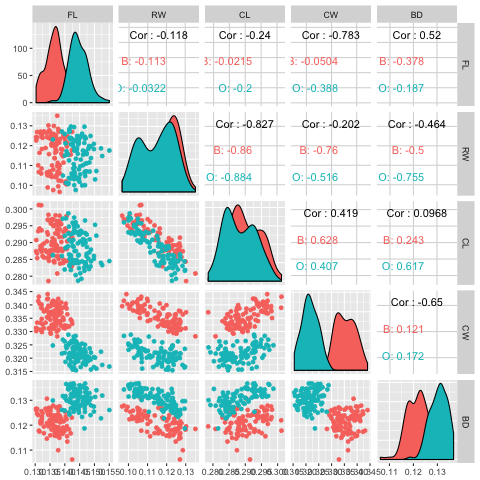
\includegraphics[width=50mm]{Figures/Crabs/matricial_plot_decorr.png}	
\captionof{figure}{Plot Matriciel des caracteristiques apres decorelation}
\label{fig:crabs_matricial_plot_decorr}
\end{center}
On remarque qu'a présent on peut visiblement distinguer les especes par leur caractéristiques Par exemple si on observe le plot de  "RW" en fonction de "CW" les espèces sont séparées.


	\begin{minipage}{.5\textwidth}
	\centering
	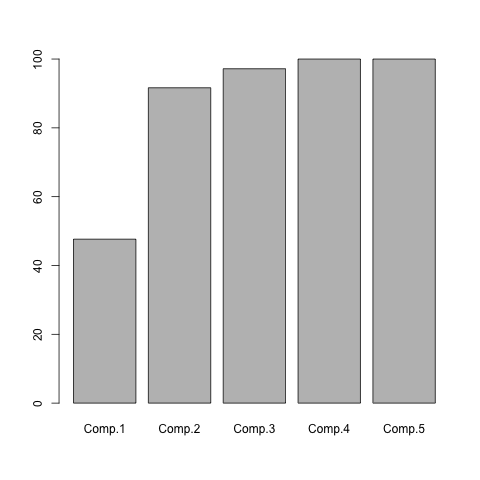
\includegraphics[width=50mm]{Figures/Crabs/decorr_pca_plot.png}
	\captionof{figure}{Variance expliquee par les composantes apres decorrelation}
	\label{fig:crabs_pca_plot}
\end{minipage}%
\hspace{0.08\linewidth}
\begin{minipage}{.5\textwidth}
	\centering
	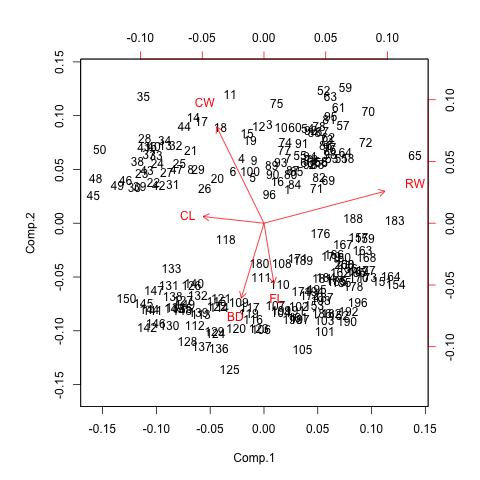
\includegraphics[width=50mm]{Figures/Crabs/decorr_pca_biplot.png}
	\captionof{figure}{Individus et Variables projetes sur le premier plan factoriel apres decorrelation}
	\label{fig:crabs_pca_biplot}
\end{minipage}


\subsection{Pima}
\subsubsection{PCA}

Nous utilisons la fonction princomp pour calculer les composantes principales dans ce dataset apres avoir centre en colonne les donnees. Ensuite nous representons le plot de la figure \ref{fig:pima_pca_plot} et le biplot de la figure \ref{fig:pima_pca_biplot}.
\\
	\begin{minipage}{.5\textwidth}
	\centering
	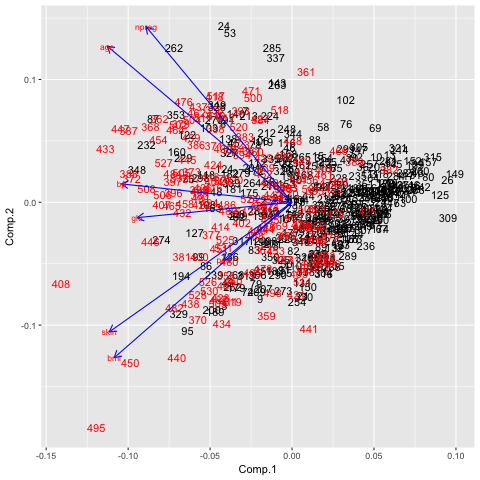
\includegraphics[width=50mm]{Figures/Pima/pca_plot.png}
	\captionof{figure}{Variance expliquee par les composantes}
	\label{fig:pima_pca_plot}
\end{minipage}%
\hspace{0.08\linewidth}
\begin{minipage}{.5\textwidth}
	\centering
	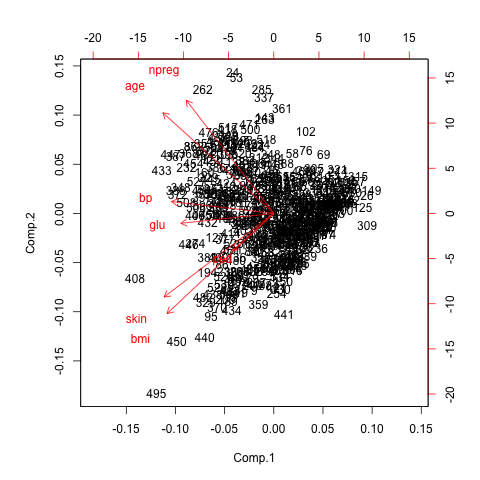
\includegraphics[width=50mm]{Figures/Pima/pca_biplot.png}
	\captionof{figure}{Individus et Variables projetes sur le premier plan factoriel}
	\label{fig:pima_pca_biplot}
\end{minipage}
\\
\\
Pour connaitre le comportement general du dataset, nous pouvons considerer les 80\% des pourcentages cumules. Dans ce cas, nous prenons 4 composantes. Si on s'interesse aux details et qu'on va jusqu'a une inertie de 95\%, on remarque qu'il faudra prendre les 6 composantes. En effet, les variables sont tres independantes et fortement decorellees. Le seul cas ou on peut avoir une representation simple est le cas general de 80\%, autrement on ne diminue pas enormement la dimension. 
\subsection{Conclusion}
>>>>>>> origin/master
\end{document}
